\documentclass[color=usenames,dvipsnames]{beamer}\usepackage[]{graphicx}\usepackage[]{color}
% maxwidth is the original width if it is less than linewidth
% otherwise use linewidth (to make sure the graphics do not exceed the margin)
\makeatletter
\def\maxwidth{ %
  \ifdim\Gin@nat@width>\linewidth
    \linewidth
  \else
    \Gin@nat@width
  \fi
}
\makeatother

\definecolor{fgcolor}{rgb}{0.345, 0.345, 0.345}
\newcommand{\hlnum}[1]{\textcolor[rgb]{0.686,0.059,0.569}{#1}}%
\newcommand{\hlstr}[1]{\textcolor[rgb]{0.192,0.494,0.8}{#1}}%
\newcommand{\hlcom}[1]{\textcolor[rgb]{0.678,0.584,0.686}{\textit{#1}}}%
\newcommand{\hlopt}[1]{\textcolor[rgb]{0,0,0}{#1}}%
\newcommand{\hlstd}[1]{\textcolor[rgb]{0.345,0.345,0.345}{#1}}%
\newcommand{\hlkwa}[1]{\textcolor[rgb]{0.161,0.373,0.58}{\textbf{#1}}}%
\newcommand{\hlkwb}[1]{\textcolor[rgb]{0.69,0.353,0.396}{#1}}%
\newcommand{\hlkwc}[1]{\textcolor[rgb]{0.333,0.667,0.333}{#1}}%
\newcommand{\hlkwd}[1]{\textcolor[rgb]{0.737,0.353,0.396}{\textbf{#1}}}%
\let\hlipl\hlkwb

\usepackage{framed}
\makeatletter
\newenvironment{kframe}{%
 \def\at@end@of@kframe{}%
 \ifinner\ifhmode%
  \def\at@end@of@kframe{\end{minipage}}%
  \begin{minipage}{\columnwidth}%
 \fi\fi%
 \def\FrameCommand##1{\hskip\@totalleftmargin \hskip-\fboxsep
 \colorbox{shadecolor}{##1}\hskip-\fboxsep
     % There is no \\@totalrightmargin, so:
     \hskip-\linewidth \hskip-\@totalleftmargin \hskip\columnwidth}%
 \MakeFramed {\advance\hsize-\width
   \@totalleftmargin\z@ \linewidth\hsize
   \@setminipage}}%
 {\par\unskip\endMakeFramed%
 \at@end@of@kframe}
\makeatother

\definecolor{shadecolor}{rgb}{.97, .97, .97}
\definecolor{messagecolor}{rgb}{0, 0, 0}
\definecolor{warningcolor}{rgb}{1, 0, 1}
\definecolor{errorcolor}{rgb}{1, 0, 0}
\newenvironment{knitrout}{}{} % an empty environment to be redefined in TeX

\usepackage{alltt}
%\documentclass[color=usenames,dvipsnames,handout]{beamer}

%\usepackage[roman]{../pres1}
\usepackage[sans]{../pres1}





\IfFileExists{upquote.sty}{\usepackage{upquote}}{}
\begin{document}



\begin{frame}[plain]
  \begin{center}
    {\Huge Extinction} \\
    \vfill
    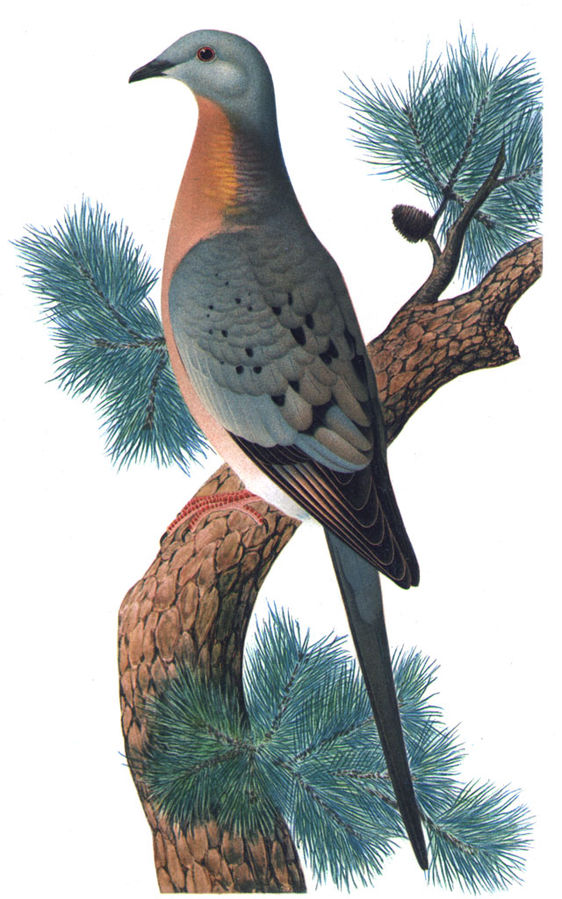
\includegraphics[height=5.5cm,keepaspectratio]{figs/passenger-pigeon} \hspace{0.5cm}
    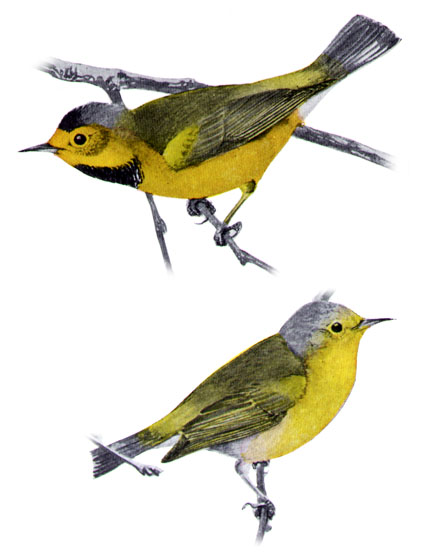
\includegraphics[height=5.5cm,keepaspectratio]{figs/Vermivora_bachmanii} %\hspace{0.1cm}
  \end{center}
\end{frame}




\section{Introduction}


\begin{frame}[plain]
  \frametitle{Learning objectives}
%  {\huge Today's topics}
  \tableofcontents%[currentsection]
\end{frame}



\begin{frame}
  \frametitle{Extinction}
  \large
%  {\bf Global}
  \begin{itemize}[<+->]
    \item Many believe that humans are causing the 6th mass extinction event
    \item At least 1000 species have gone extinct over past 500 years
    \item Extinction rate unknown, but may be 100-1000 times higher
      than during the past 25 million years
    \item Almost 200 bird species have gone extinct since 1500
    \item Avian extinctions in GA: passenger
      pigeon, Bachman's warbler, ivory-billed woodpecker, Carolina parakeet
  \end{itemize}
  \uncover<6->{
  \begin{center}
    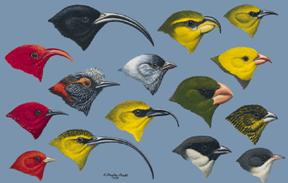
\includegraphics[height=2.5cm,keepaspectratio]{figs/bird-radiation}
    \\ %\hspace{0.5cm}
    \vfill \tiny
% \url{
%    http://www.discovery.com/tv-shows/racing-extinction/the-song-of-the-last-kauai-oo-bird/
%  } \\
    \url{
      https://vimeo.com/42592260
    }
  \end{center}
  }
\end{frame}



\begin{comment}
\begin{frame}
  \frametitle{}
BBC series -- Extinction: The Facts
% {https://www.bbc.co.uk/programmes/p08rg347} % overview
  \url{
    https://www.bbc.co.uk/programmes/p08qy8lr % brief overview
  }
  \url{
    https://www.bbc.co.uk/programmes/p08qym98 % vortex
  }
  \url{
    https://www.bbc.co.uk/programmes/p08qy8lz % last white rhino
  }
  \url{
    https://www.bbc.co.uk/programmes/p08qym6s % giraffe
  }
Hawaii
  \url{
    https://vimeo.com/42592260 % 
  }
  \url{
    https://youtu.be/J0UlrJeW8n8 % Hawaii birds
  }
\end{frame}
\end{comment}


% \begin{frame}
%   \frametitle{Correlates of extinction risk}
%   \Large
%   {Species with high extinction risk often have:}
%   \begin{itemize}
% %%    \item<2-> Body size?
%     \item<2-> Small range
%     \item<2-> Low population size
%     \item<2-> Limited dispersal ability
%     \item<2-> Low population growth rate
% %%    \item<2-> Long generation time
% %%    \item<2>  Environmental stochasticity
%   \end{itemize}
% \end{frame}







\section{Deterministic Models}



%% \begin{frame}
%%   \frametitle{Why do we need models?}
%%   Time to extinction
%%   Extinction risk
%% \end{frame}



\begin{frame}
  \frametitle{Deterministic models}
  \Large
%   \begin{itemize}[<+->]
%     \item For a model with no random variation, \textit{time to extinction} can
%       be calculated easily
%     \item But how should we define extinction?
%     \item Time to quasi-extinction ($T_e$) is time it takes for a
%       population to reach an extinction threshold beyond which it is doomed
%     \item Threshold usually based on genetic considerations, Allee
%       effects, etc\dots
% %    \item Usually, people talk about quasi-extinction, which is some
% %        population size below which the population is likely doomed.
% %    \item Quasi-extinction threshold decision usually based on genetic
% %      considerations, Allee effects, etc\dots
%   \end{itemize}
  For a model with no random variation, \textit{time to extinction} can
      be calculated easily. \\
  \pause \vfill
  But how should we define extinction? \\
  \pause \vfill
  Time to quasi-extinction ($T_e$) is the time it takes for a
      population to reach an extinction threshold beyond which it is
      doomed. \\
  \pause \vfill
  Threshold usually based on genetic considerations, Allee
      effects, etc\dots
\end{frame}





\begin{frame}[fragile]
  \frametitle{Geometric growth example}
%  \vspace{-0.4cm}
%  \begin{center}

%\end{center}
\includegraphics[width=\textwidth]{figure/exp1-1}
\end{frame}



%\begin{frame}
%  \frametitle{Population viability analysis}
%  A PVA seeks to determine effects of managment actions or environmental
%  change on time to quasi-extinction ($T_e$)
%  \pause
%  Deterministic models clearly aren't realistic
%\end{frame}





\section{Stochastic Models}




%% \begin{frame}
%%   \frametitle{Stochastic}
%%   {\bf Environmental stochasticity}
%%   \begin{itemize}
%%     \item Random variation in weather, habitat, etc\dots among years
%%     \item[]
%%   \end{itemize}
%%   \pause
%%   {\bf Demographic stochasticity}
%%   \begin{itemize}
%%     \item Random variation in the number of births or deaths in among years
%%     \item[]
%%   \end{itemize}
%% \end{frame}






\begin{frame}
  \frametitle{Extinction risk}
  \Large
  % \begin{itemize}
  %   \item In addition to time to extinction ($T_e$), we are now
  %     interested in \textit{extinction risk}
  %   \item<2-> Extinction risk is the \textit{probability} that a species goes
  %     extinct in some time period
  %   \item<3-> For a stochastic model, extinction risk can be
  %     calculated as the proportion of simulations in which the
  %     population goes extinct.
  %   \item<4-> Calculating extinction risk requires a specification of
  %     the time horizon of interest
  % \end{itemize}
  In addition to time to extinction ($T_e$), we are now
  interested in \textit{extinction risk}. \\
  \pause \vfill
  Extinction risk is the \textit{probability} that a species goes
  extinct in some time period. \\
  \pause \vfill
  For a stochastic model, extinction risk can be
  calculated as the proportion of simulations in which the
  population goes extinct. \\
  \pause \vfill
  Calculating extinction risk requires a specification of
  the time horizon of interest.
\end{frame}









\begin{frame}
  \frametitle{Logistic growth with stochastic carrying capacity}
  \LARGE
\[
  N_{t+1} = N_t + N_tr_{max}(1 - N_t/K_t)
\]

\vspace{0.3cm}
{\large \centering where \par}
\[
  K_t \sim \mbox{Normal}(\bar{K}, \sigma_e^2)
\]
\end{frame}






\begin{frame}[fragile]
  \frametitle{Logistic example, $r_{max}=0.3$, $\bar{K}=100$, $\sigma_e^2=400$}

\vspace{0.0cm}
\begin{center}
  \includegraphics<1 | handout:0>[width=\textwidth]{figs/lg-d/lg-d1}
  \includegraphics<2 | handout:0>[width=\textwidth]{figs/lg-d/lg-d2}
  \includegraphics<3 | handout:0>[width=\textwidth]{figs/lg-d/lg-d3}
  \includegraphics<4 | handout:0>[width=\textwidth]{figs/lg-d/lg-d4}
  \includegraphics<5 | handout:0>[width=\textwidth]{figs/lg-d/lg-d5}
  \includegraphics<6 | handout:0>[width=\textwidth]{figs/lg-d/lg-d6}
  \includegraphics<7 | handout:0>[width=\textwidth]{figs/lg-d/lg-d7}
  \includegraphics<8 | handout:0>[width=\textwidth]{figs/lg-d/lg-d8}
  \includegraphics<9 | handout:0>[width=\textwidth]{figs/lg-d/lg-d9}
  \includegraphics<10>[width=\textwidth]{figs/lg-d/lg-d100}
\end{center}
\end{frame}





\begin{frame}
  \frametitle{Extinction risk}
  {Zero extinctions in 100 simulations, hence extinction risk is
    (approximately) zero over the 20 year time horizon \par}
  \vfill
  \pause
  {Assumptions}
  \begin{itemize}
    \item We have the correct model
    \item We know the parameters with certainty
  \end{itemize}
%%  \pause
%%  \vfill
\end{frame}





\begin{frame}[fragile]
  \frametitle{Logistic example, $r_{max}=0.3$, $\bar{K}=100$, $\sigma_e^2=1600$}

\vspace{0.0cm}
\begin{center}
  \includegraphics<1 | handout:0>[width=\textwidth]{figs/lg-d/lg2-d1}
  \includegraphics<2 | handout:0>[width=\textwidth]{figs/lg-d/lg2-d2}
  \includegraphics<3 | handout:0>[width=\textwidth]{figs/lg-d/lg2-d3}
  \includegraphics<4 | handout:0>[width=\textwidth]{figs/lg-d/lg2-d4}
  \includegraphics<5 | handout:0>[width=\textwidth]{figs/lg-d/lg2-d5}
  \includegraphics<6 | handout:0>[width=\textwidth]{figs/lg-d/lg2-d6}
  \includegraphics<7 | handout:0>[width=\textwidth]{figs/lg-d/lg2-d7}
  \includegraphics<8 | handout:0>[width=\textwidth]{figs/lg-d/lg2-d8}
  \includegraphics<9 | handout:0>[width=\textwidth]{figs/lg-d/lg2-d9}
  \includegraphics<10>[width=\textwidth]{figs/lg-d/lg2-d100}
\end{center}
\end{frame}








%% \begin{frame}
%%   \frametitle{Extinction risk}
%%   17 extinctinos in 100 simulations.
%% \end{frame}



\section{Allee effects}



\begin{frame}
  \frametitle{Allee effects}
  {Normally, population growth rates increase as the population
    decreases (negative correlation) \par}
  \pause
  \vfill
  {The Allee effect is the phenomenon of positive correlation
    between population growth rates and population size \par}
  \pause
  \vfill
  {Mechanisms}
  \begin{itemize}
    \item Finding a mate becomes difficult
    \item Social systems collapse
    \item Inbreeding depression
    \item etc\dots
  \end{itemize}
  \pause
  \vfill
  {Allee effects can greatly increase extinction risk for small populations}

\end{frame}



\begin{frame}[fragile]
  \frametitle{Allee effects}

%\begin{center}
  \begin{columns}
    \column{\dimexpr\paperwidth-10pt}
  \includegraphics[width=\textwidth]{figure/Allee-1}
  \end{columns}
%\end{center}
\end{frame}









%% \begin{frame}[fragile]
%%   \frametitle{Logistic example with Allee effects}
%%   \note{Change this example}
%% <<fig=FALSE,echo=FALSE>>=
%% r.max <- 0.3
%% K.bar <- 100
%% sigma.d <- 40
%% T <- 20
%% set.seed(4450)
%% ##plot(0:T, N, type="b", xlab="Time", ylab="Population size (N)",
%% ##     ylim=c(0, 300))
%% nSim <- 100
%% N <- Nlr <- matrix(NA, T+1, nSim)
%% N[1,] <- Nlr[1,] <- 25
%% Te <- integer(nSim)
%% Tes <- NULL
%% for(i in 1:nSim) {
%%     fl <- paste("figs/lg-d/lg3-d", i, ".pdf", sep="")
%%     for(t in 1:T) {
%%         K.t <- rnorm(1, K.bar, ifelse(N[t,i]<50, 80, sigma.d))
%%         r.prime <- r.max ##ifelse(N[t,i] < 50, 0.1, r.max)
%%         N[t+1,i] <- N[t,i] + N[t,i]*r.prime*(1 - N[t,i]/K.t)
%%         N[t+1,i] <- N[t+1,i]*(N[t+1,i]>0)
%%         Nlr[t+1,i] <- Nlr[t,i] + Nlr[t,i]*r.max*(1 - Nlr[t,i]/K.bar)
%%     }
%%     ext <- N[,i]<1
%%     if(any(ext)) {
%%         Te[i] <- min(which(ext))-1
%%         Tes <- which(Te>0)
%%     }
%%     if(i < 11 || i==nSim) {
%%         pdf(fl, width=8, heigh=6)
%%         par(mai=c(0.9,0.9,0.3,0.3))
%%         mn <- ifelse(i==nSim, paste(nSim, "Simulations"), "")
%%         matplot(0:T, N, type="l", xlab="Time", ylab="Population size (N)", main=mn,
%%              ylim=c(0, 150), col=gray(0.7), lty=1, cex.lab=1.5)
%%         lines(0:T, Nlr[,1], col="blue", lwd=3)
%%         abline(h=0, col="red", lwd=2)
%%         points(Te[Tes], rep(0, length(Tes)), pch=16, col="orange", cex=1.5)
%%         dev.off()
%%     }
%% }
%% @
%% \vspace{0.0cm}
%% \begin{center}
%%   \includegraphics<1 | handout:0>[width=0.7\textwidth]{figs/lg-d/lg3-d1}
%%   \includegraphics<2 | handout:0>[width=0.7\textwidth]{figs/lg-d/lg3-d2}
%%   \includegraphics<3 | handout:0>[width=0.7\textwidth]{figs/lg-d/lg3-d3}
%%   \includegraphics<4 | handout:0>[width=0.7\textwidth]{figs/lg-d/lg3-d4}
%%   \includegraphics<5 | handout:0>[width=0.7\textwidth]{figs/lg-d/lg3-d5}
%%   \includegraphics<6 | handout:0>[width=0.7\textwidth]{figs/lg-d/lg3-d6}
%%   \includegraphics<7 | handout:0>[width=0.7\textwidth]{figs/lg-d/lg3-d7}
%%   \includegraphics<8 | handout:0>[width=0.7\textwidth]{figs/lg-d/lg3-d8}
%%   \includegraphics<9 | handout:0>[width=0.7\textwidth]{figs/lg-d/lg3-d9}
%%   \includegraphics<10>[width=0.7\textwidth]{figs/lg-d/lg3-d100}
%% \end{center}
%% \end{frame}





\begin{frame}
  \frametitle{Summary}
  \large
%   \begin{itemize}
%     \item Humans have increased extinction rates dramatically
%     \item Models allow us to predict time to extinction and extinction risk
% %    \item Models allow us to identify concerns such as Allee effects
%     \item Models can be used to assess effects of management actions on extinction risk
%   \end{itemize}
   Humans have increased extinction rates dramatically. \vfill
   Models allow us to predict time to extinction and extinction risk. \vfill
   Models can be used to assess effects of management actions on
   extinction risk. \vfill
\end{frame}



\begin{frame}
  \frametitle{Assignment}
  \LARGE
  \centering
  Read pages 27--31 in Conroy and Carroll \par
\end{frame}




\end{document}


